\documentclass{beamer}

% THEME (Metropolis)
\usetheme[numbering=counter,progressbar=foot]{metropolis} % clean + progress bar
\usepackage{appendixnumberbeamer}

% FONTS (works with pdfLaTeX; for nicer system fonts, compile with XeLaTeX)
\usepackage[T1]{fontenc}
\usepackage[utf8]{inputenc}
\usepackage{lmodern}

% MATH / GRAPHICS
\usepackage{amsmath, amssymb}
\usepackage{graphicx}
\graphicspath{{figures/}} % put your figures in ./figs

% BIB (optional) — comment out if not needed
\usepackage[numbers]{natbib}
\usepackage{bibentry}

% TITLE INFO
\title{Scalability and Communication Overhead in Distributed N-Body Simulation using MPI on GCP}
\author{Your Name}
\institute{Your Dept. / University}
\date{\today}

\begin{document}

% TITLE SLIDE
\maketitle

% AGENDA
\begin{frame}{Outline}
  \tableofcontents
\end{frame}

\section{Problem \& Model}
\begin{frame}{N-Body Problem (Direct Method)}
  \begin{itemize}
    \item $N$ point masses, gravitational interaction only.
    \item Direct method: compute all pairwise forces $\Rightarrow O(N^2)$.
    \item Parallelization goal: distribute bodies and keep a global view of positions.
  \end{itemize}
  \vspace{0.5em}
  \textbf{Key equation:}
  \[
    \vec{a}_i=\sum_{\substack{j=0 \\ j \neq i}}^{N-1}
    \left[G\frac{m_j}{\|\vec{r}_i-\vec{r}_j\|^3}(\vec{r}_j-\vec{r}_i)\right]
  \]
\end{frame}

\section{Method}
\begin{frame}{MPI Parallelization at a Glance}
  \begin{columns}[T,totalwidth=\textwidth]
    \column{0.55\textwidth}
    \begin{itemize}
      \item Bodies split across $P$ processes ($\approx N/P$ each).
      \item Each step:
      \begin{enumerate}
        \item Allgather positions (and once masses).
        \item Compute local accelerations.
        \item Update velocities/positions.
      \end{enumerate}
      \item Uses \texttt{MPI\_Allgatherv} (blocking, collective).
    \end{itemize}
    \column{0.42\textwidth}
    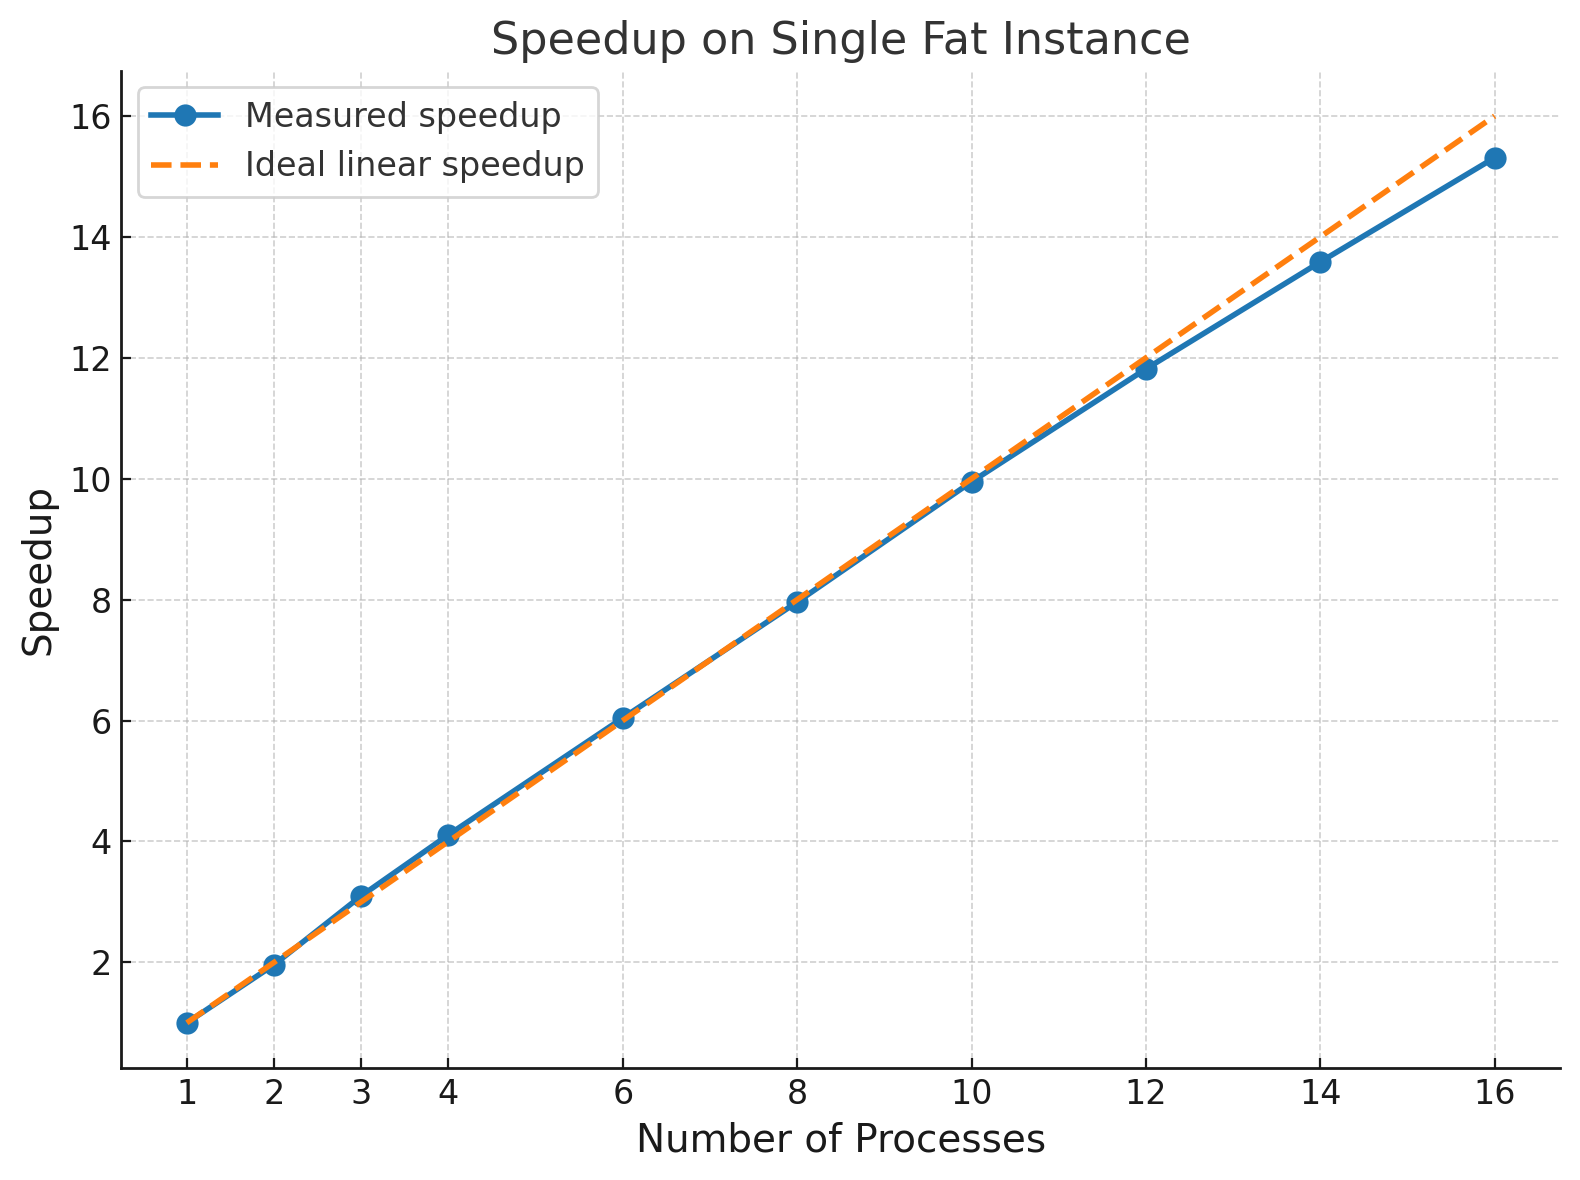
\includegraphics[width=\linewidth]{parallel_strong_scaling_16_cores.png}
    \vspace{0.3em}
    \scriptsize Example plot placeholder
  \end{columns}
\end{frame}

\section{Results}
\begin{frame}{Strong Scalability (Single Fat Instance)}
  \begin{itemize}
    \item Near-linear speedup up to 16 processes on one VM.
    \item Communication time is negligible intra-node.
  \end{itemize}
  \vspace{0.5em}
  \centering
  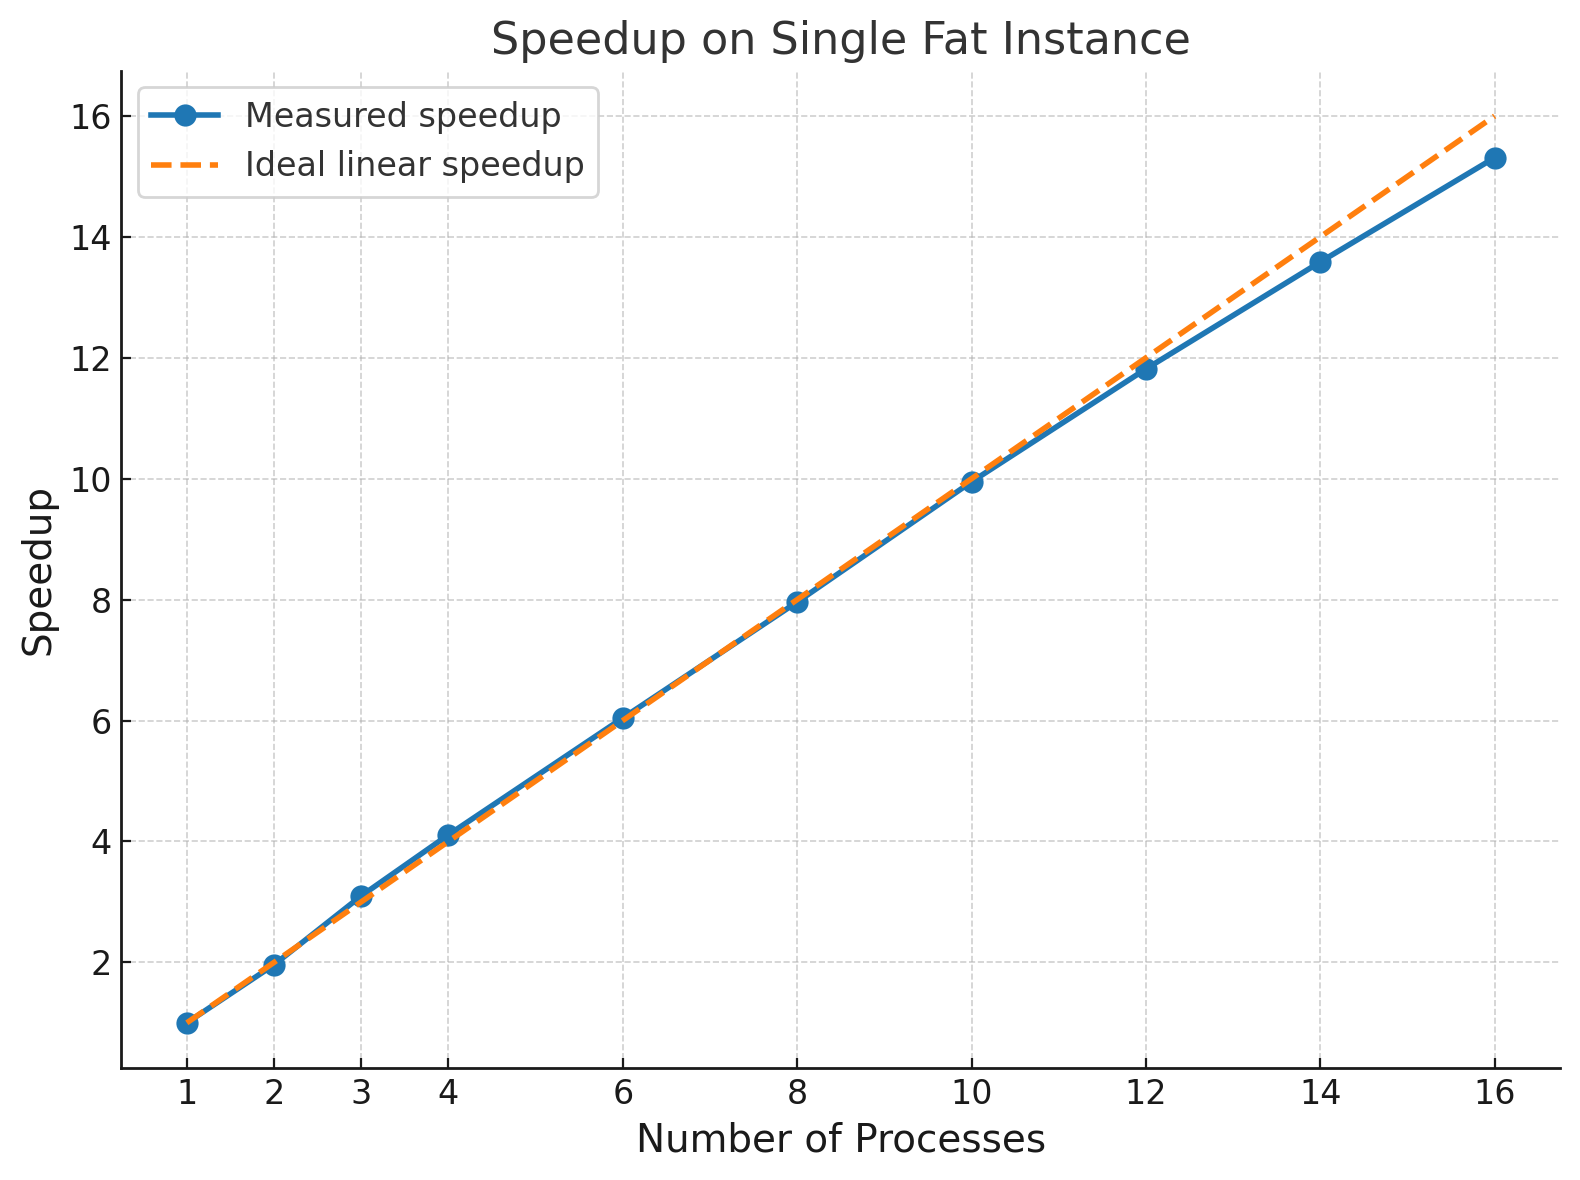
\includegraphics[width=0.8\linewidth]{parallel_strong_scaling_16_cores.png}
\end{frame}

\begin{frame}{Communication Overhead Across Configurations}
  \begin{itemize}
    \item Intra-regional clusters: modest overhead.
    \item Inter-regional / multi-region: \texttt{MPI\_Allgatherv} becomes dominant.
  \end{itemize}
  \centering
  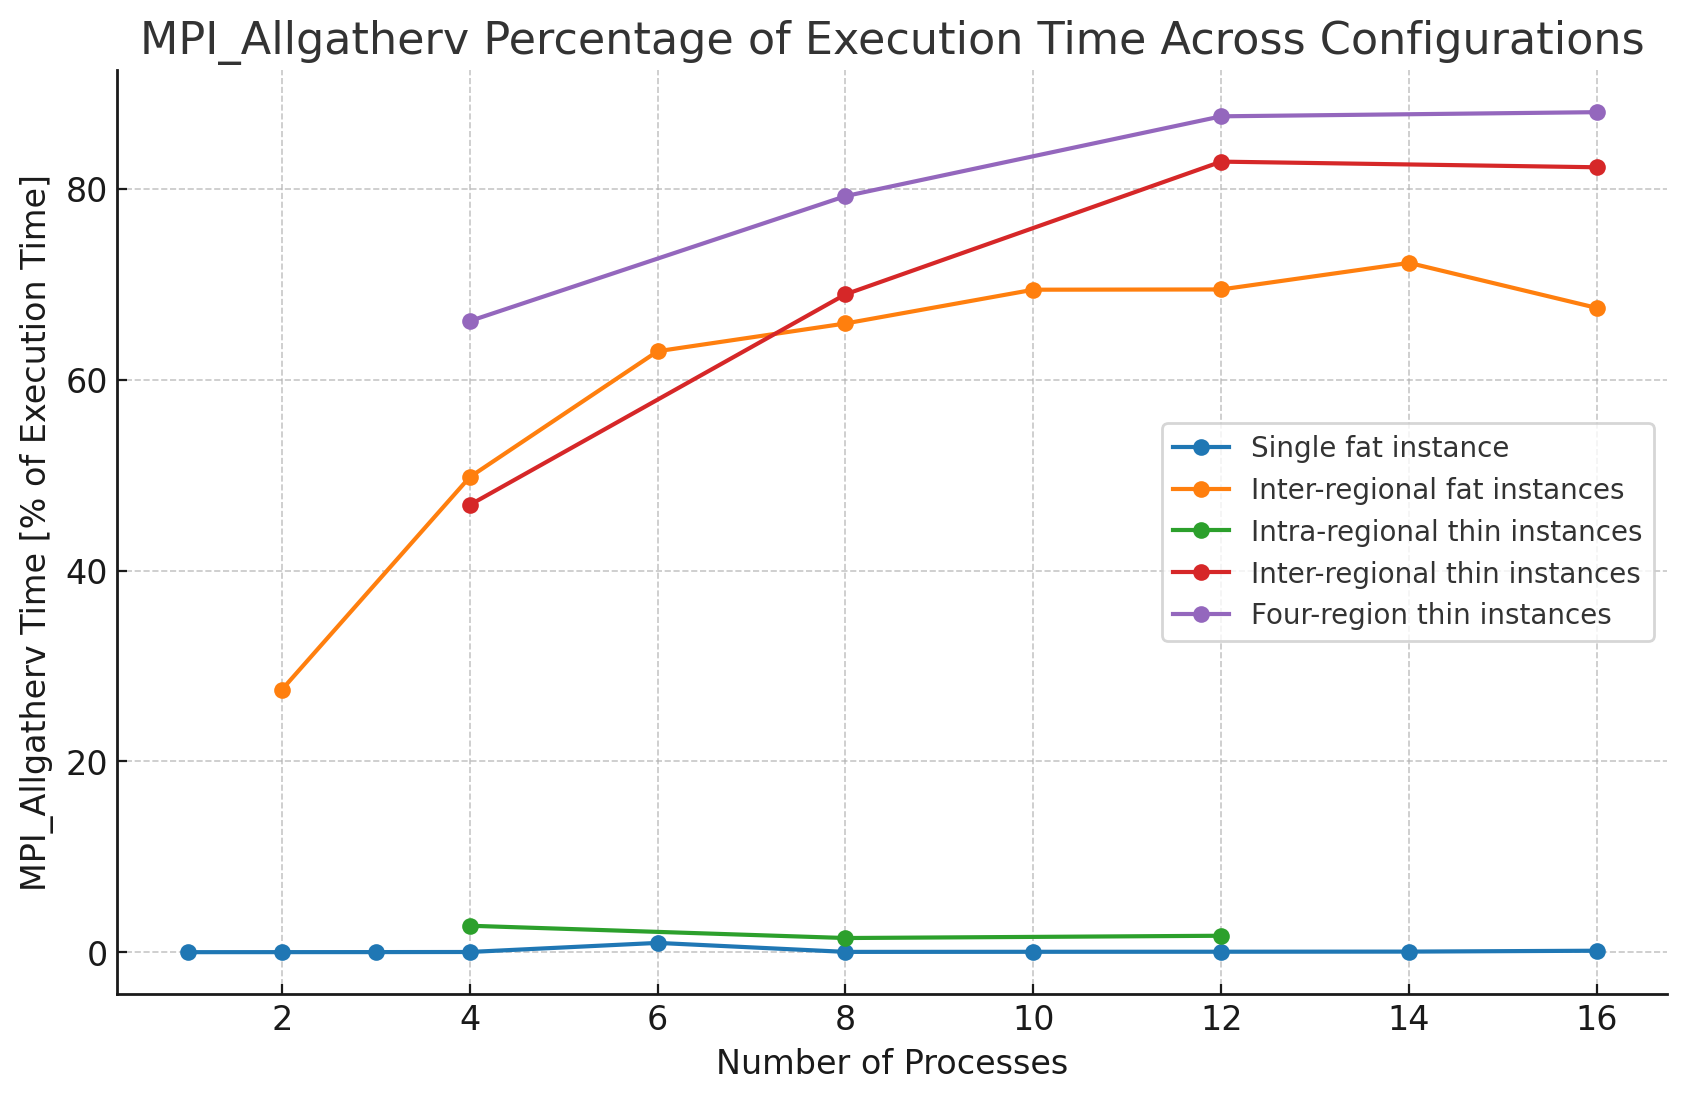
\includegraphics[width=0.85\linewidth]{communication_fraction_ex_time.png}
\end{frame}

\begin{frame}{Weak Scalability (Direct Method)}
  \begin{itemize}
    \item With $N \propto P$, per-process data is constant, but
    \item Per-process \emph{computational} work $\sim O(N^2/P)\propto P$.
    \item Runtime grows with $P$ (poor weak scalability).
  \end{itemize}
  \centering
  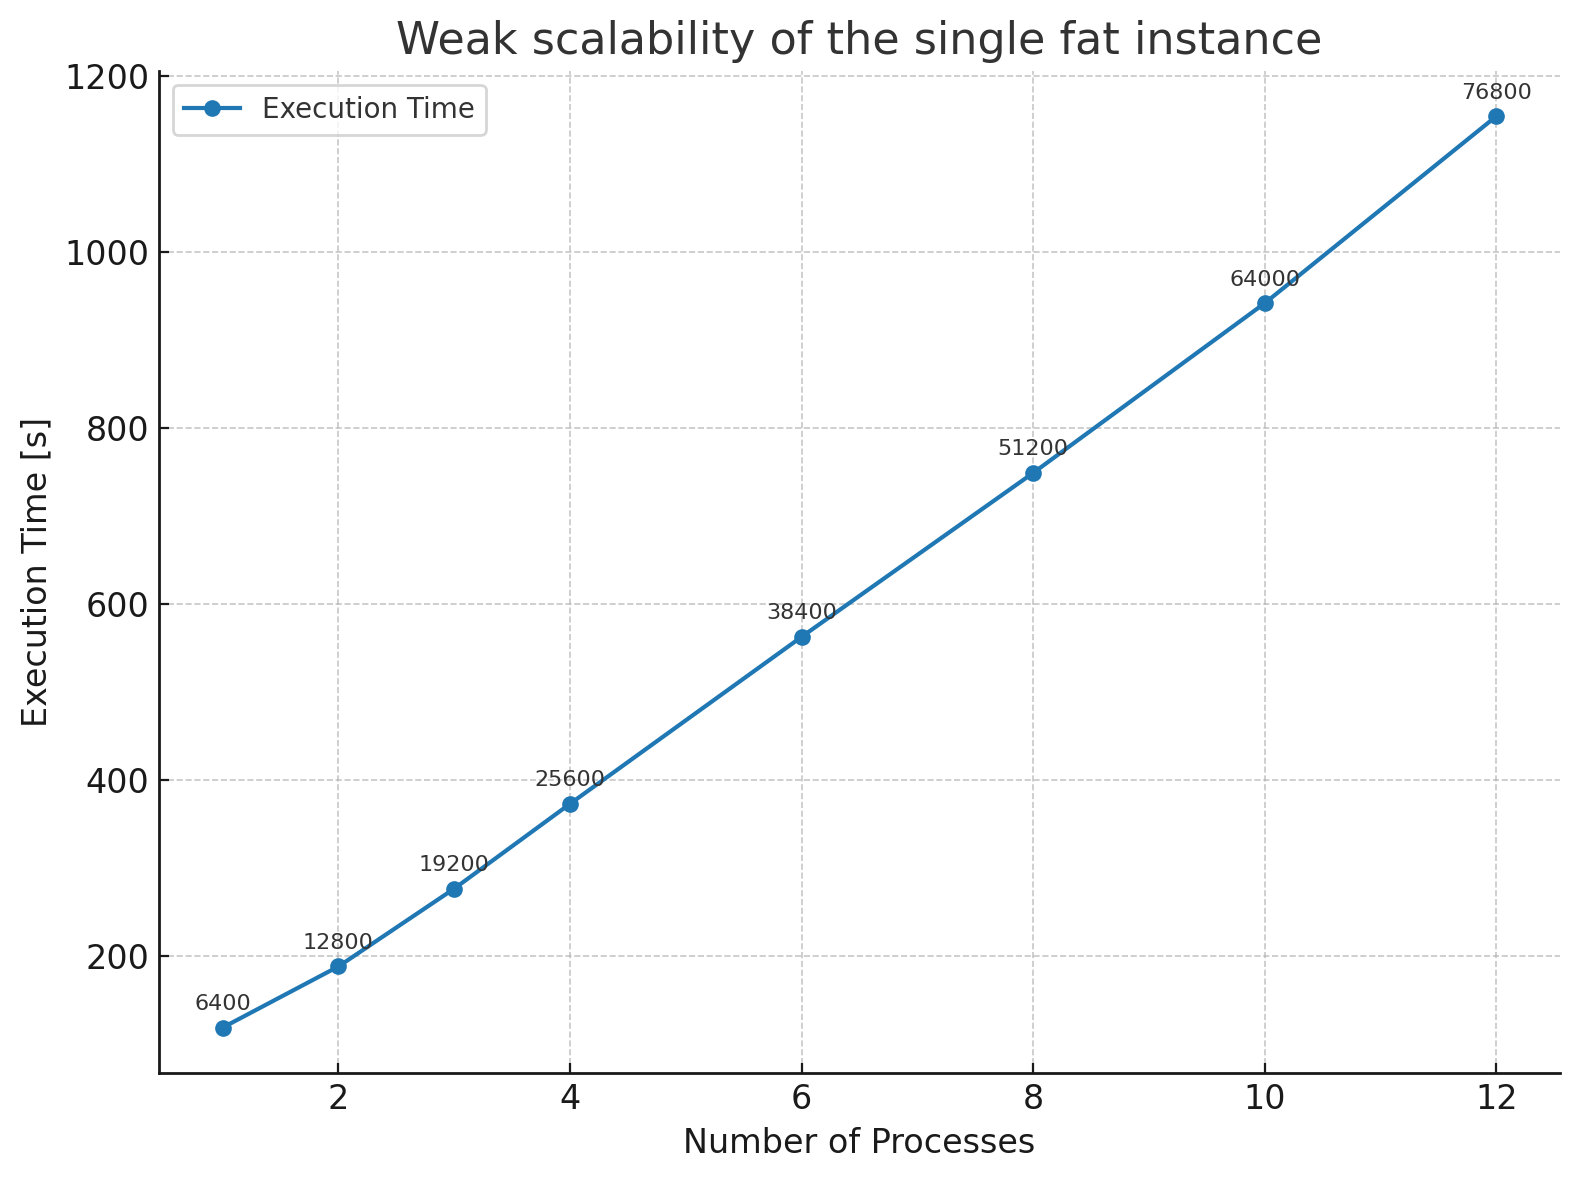
\includegraphics[width=0.8\linewidth]{parallel_weak_scalability.png}
\end{frame}

\section{Takeaways}
\begin{frame}{Conclusions}
  \begin{itemize}
    \item Strong scalability holds intra-node / intra-region.
    \item Inter-region latency breaks scalability (blocking collective).
    \item Direct $O(N^2)$ method limits weak scalability.
    \item Future work: hierarchical/approximate methods (e.g., Barnes--Hut).
  \end{itemize}
\end{frame}

\begin{frame}[standout]
  Questions?
\end{frame}

% OPTIONAL: References slide
% \begin{frame}[allowframebreaks]{References}
%   \small
%   \bibliographystyle{unsrtnat}
%   \bibliography{references}
% \end{frame}

\end{document}

